\section{Methodology}\label{ch4:sec:Methodology}


This section describes the methods, beginning with data collection, followed by the training of the RL-agent and the deployment of the algorithm. To the best of our knowledge, this paper is the first to use an offline RL to train an agent to dynamically regulate the power of a datacenter/HPC cluster node. The different phases of the approach are depicted pictorially in Figure~\ref{ch4:fig:flow-diagram}. As shown in the figure, there are no closed loops between the RL agent and the evaluation process, meaning the agent is trained without feedback from direct interaction with the target system.

\begin{figure}[htb]
    \centering
    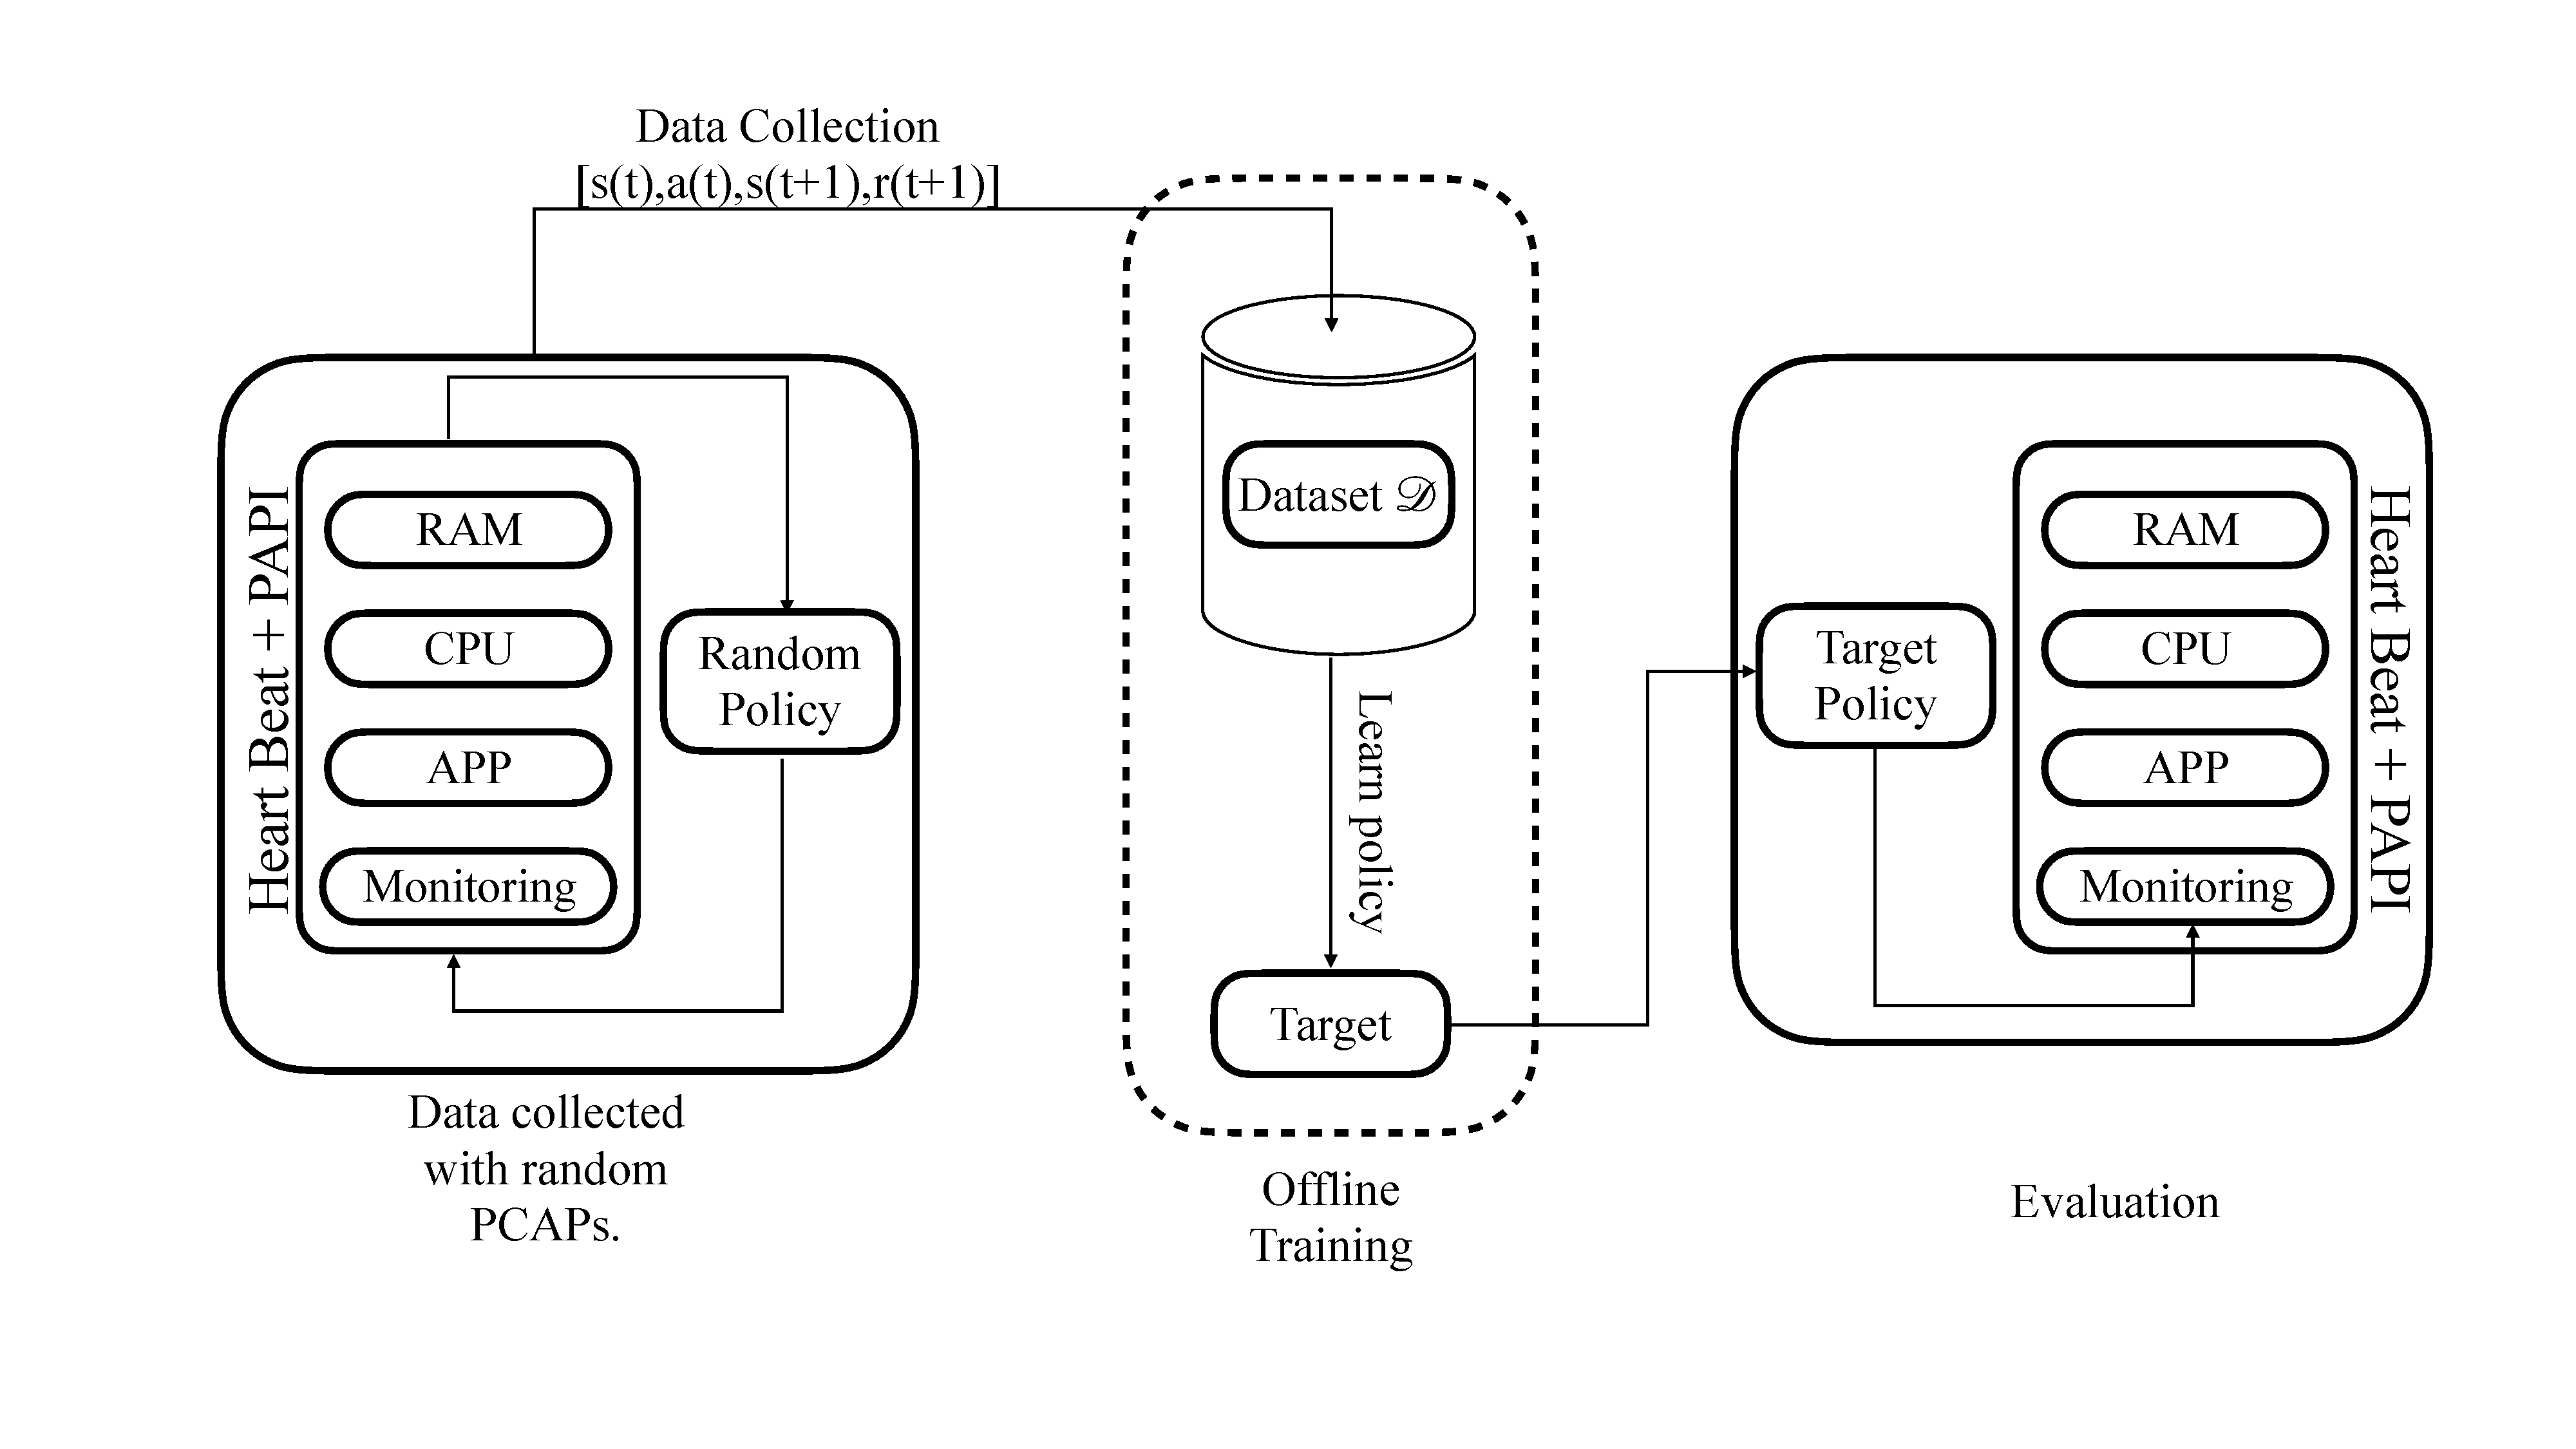
\includegraphics[width=.9\linewidth,trim=5.5cm 6cm 3cm 1cm]{Figures/block_diagram.pdf}
    \caption{{Flow diagram for offline reinforcement learning: data is collected using an arbitrary policy to train the agent without system  , and the trained agent is later deployed for evaluation. Note that the lines in the diagram are not closed to form a loop, indicating offline training and online testing.}}
    \label{ch4:fig:flow-diagram}
%    \Description{Flow diagram of methodology}
\end{figure}

% Akhilesh, moved this subsection from Background to here and gave it a specific subheading
\subsection{Dataset Collection: Capturing Application Performance through Hardware Performance Counters} \label{ch4:subsec:Applications_vs_perf}

Unlike existing works \cite{10305814} that use a mathematical model to describe the relationship between application performance and power for training an RL agent, our approach learns directly from a collected dataset, which consists of performance and power data. By analyzing a set of pre-collected data, the RL agent aims to improve decision-making processes and optimize performance over the course of training iterations. 

Dataset collection itself is a challenging problem because 
different applications can illustrate differing performance on a given hardware architecture.
This performance is influenced by hardware characteristics such
as memory bandwidth, CPU cores, and cache size. To capture this complex
application-hardware interaction in our dataset, we leverage a set of hardware performance
counters while running applications on the target system. Specifically, we rely on the
Performance Application Programming Interface (PAPI)~\cite{mucci1999papi} to provide portable access to hardware performance counters.  PAPI offers easy access to a variety of counters through direct queries on the hardware model-specific registers. These measurements are representative of hardware-specific and application-specific data movement, or a combination of both.

To optimize energy efficiency while preserving performance, we focus on a small set of key performance metrics: total instructions issued ($TOT\_INS$), total clock cycles ($TOT\_CYC$), total last-level cache accesses ($L3\_TCA$), last-level cache misses ($L3\_TCM$), and cycles stalled because of resource contention ($RES\_STL$). We chose these key metrics for two reasons. First, these readings are available instantaneously and simultaneously during every sampling interval. Second, they are direct and sufficient indicators of the rate of data flow within and between the CPU cores and memory. Furthermore, because direct usage of these metrics would call for a large trained network and necessitate additional data processing, we follow insights from other research~\cite{wittmann2016chip,rane2014enhancing} in computing a set of \textit{derived metrics} (instructions per cycle ($IPC$), the ratio of stalled cycles to total cycles (often equated with CPU utilization, noted as $STL$), and last-level cache miss rate ($CMR$)) which facilitate a more detailed analysis of runtime behavior.  

\textbf{Key Insight:} Based on findings from previous works, we note that these metrics should not be viewed in isolation as definitive indicators of performance, since varying IPC values, for example, can still lead to the same execution time. Nonetheless, these derived metrics serve as valuable proxies to discern application characteristics, including its arithmetic intensity or whether the application is memory-bounded and thus can operate efficiently within a lower power budget.

% Benchmark applications are widely used to evaluate and rank system performance. They are also important in understanding how the computations can scale with the changes in number of nodes/ cores thereby using the appropriate setup for future experiments. For example, one of the applications that we use for our experiments, the STREAM benchmark, \cite{mccalpin1995memory} is designed to understand the effect of memory bandwidth on performance. It consists of four kernels namely add, copy, scale and triad (a combination of remaining three kernels), constantly querying the memory for the assigned operation with a query size equivalent to the problem size given as input. The latency of this execution depends on the time it takes for the application to retrieve this information from the memory and can be accumulate over iterated execution of the same process. Similarly there are compute bound benchmark applications, such as NAS Parallel benchmark applications (NAS) \cite{10.1145/125826.125925}, that are limited in performance by the CPU frequency. We use six of the eight benchmark applications (remaining two are used in testing) with carefully chosen problem size, enough to saturate the CPU and memory, for data collection and evaluation. Each kernel takes a finite but shorter run time for its execution. This execution time is not sufficient to capture the latency imposed by the memory bandwidth. Therefore we add iterations to each of these kernels to sustain the queries of the CPU on memory thereby accumulating the latency. This will be reflected on the total execution time of each of the application and also on the corresponding performance counter measurements. \todo{badly explained, needs rework}
% Table \ref{ch4:tab:performance_metrics} presents the characteristics of various benchmark applications used throughout this paper. We include the problem size, iterations, average $IPC$, average $CMR$, average $STL$, average $progress$ and average execution time ($ET$) for each kernel, calculated over 10 independent runs. 
% We use these features mentioned in the Table \ref{ch4:tab:performance_metrics} as the runtime characteristics of the application running on a node which goes into the state definition. The power supplied to the node is regulated using the power cap parameter, $PCAP(t)$. The allowed values of $PCAP(t)$ varies with hardware architecture. 
% Moving to the experimental setup

% 
%%%%%%%%%%%%%%%%

% Akhilesh, this was the second subsection from Background that I moved here. 
\subsection{Augmenting the Dataset with Application Progress} \label{ch4:subsec:Performance_Measurement}
To train the RL model, we must define the observables that constitute the states. In our case, we represent one aspect of the state of the RL agent related to application behavior, which is identified through hardware performance counters using the data collection steps shown above. Additionally, the instantaneous performance of the application and useful work it does, measured through application instrumentation, and the ongoing power consumption are also integral to the state. These characteristics can vary across applications.
%and can be visualized by using the values provided in Table~\ref{ch4:tab:performance_metrics}.

We augment our monitoring of application behavior by adding a notion of application \textit{progress}, or \textit{heartbeats}, to our system. This measure is obtained by a lightweight instrumentation of the applications under study.  Our approach follows the work of Ramesh et al.~\cite{ramesh2019understanding} and follows the instrumentation steps outlined by Cerf et al.~\cite{cerf2021sustaining}.
The role of this progress measurement is to highlight the potential for an application to be busy-waiting for some resource in the system and thus be showing up as being active but in reality is not making useful use of compute power.

We redefine the progress measurement equation introduced in~\cite{ramesh2019understanding} by considering the number of heartbeats received between two sampling (control) instants. The progress at time instant $t_i$ is given by Equation~\eqref{ch4:eq:progress-calculation}:

\begin{equation}
\begin{aligned}
progress(t_i) = \underset{\forall k,t_k \in [t_{i-1},t_i]}{\text{median}}\bigg(\frac{N}{t_k-t_{k-1}} \bigg),
\end{aligned}
\label{ch4:eq:progress-calculation}
\end{equation}
where $N$ represents the number of heartbeats received between the time instants
$t_k$ and $t_{k-1}$. This measure of
progress can be understood as a proxy for monitoring the figure of merit
of an application at runtime. Equation~\eqref{ch4:eq:progress-calculation} enables us to accurately measure progress while considering the time interval and the number of heartbeats received. It also allows us to limit the heartbeat-rate of instrumentation to avoid overflowing our infrastructure with messages, since  it is sufficient to accumulate a 
heartbeat counter on the application side and to only periodically send this
counter to our data collection and control infrastructure. 

\subsection{Training the RL Agent using Offline Collected Dataset}\label{ch4:sec:training}
% Akhilesh, I added the above subsection with specific heading to convey what is in these
% below paras.
The resulting collected dataset consists of quadruples of state, action, next state, and reward, corresponding to different benchmarks (training/testing). 


%%%%%%%%%% move to experimental setup
%The action space is a discretization of the range of power caps supported by the hardware, in this case the TDP value of Intel processor we use for our experiments results in 16 $PCAP$ for the RAPL actuators.
%%%%%%%%%%%%

Our objective, as defined in Section~\ref{ch4:sec:Problem}, is to identify the maximum efficiency point ($\max{PPW}$) of operation for the application on a compute node, which will be represented by a suitable reward function. The reward function in RL helps the agent learn a policy that aligns with the optimization goal. In our case, the reward should be a function of application progress and power consumption, which together constitute $PPW$ (performance per watt). The reward function $r(t)$ is thus defined as
%\vspace{-0.2cm}
\begin{equation}
\begin{aligned}
reward(t+1) = \frac{progress^3(t+1)}{P_{avg}(t+1)+1e^{-3}},
% reward(t+1) = \frac{progress(t+1)}{\frac{PCAP(t)^2}{power(t+1)}+power(t+1)},
\end{aligned}
\label{ch4:eq:reward_function}
\end{equation}
%
where the reward is an explicit function of $progress(t+1)$ and $P_{avg}(t+1)$ representing the progress and measured power, respectively. A small constant (0.001) is added to the denominator to avoid division by 0. The rest of the notations follow the earlier definitions. The overall structure of the reward function is designed to maximize the reward for improved progress while penalizing high actual power consumption. The $progress(t+1)$ term cubed in the numerator shows that more progress leads to a higher reward. 
% Akhilesh,  there is no PCAP term in the above eqn. Where is the squared pcap term that is referenced?
The squared $PCAP(t)$ in the denominator suggests that the reward decrease is more than proportional to the increase in input power; thus, using significantly more input power than necessary reduces the reward substantially. 
% The $power(t+1)$ term is penalized in two ways: first, inversely with respect to the input power, encouraging careful management of input power relative to consumption, and second, directly adding it, suggesting that the system penalizes inefficiencies or wastefulness. 

% Akhilesh, this following para is too abstract. How to tie it to our dataset?
We note that in CQL the reward is part of the dataset and can be calculated before training, since it is a function of the next state and measured power.
The state variables include characteristics that provide insights into potential bottlenecks occurring during the application runtime. The reward function determines the efficiency or quality of $PCAP$ deployed to achieve the measured state. 
% Therefore, training the RL agent allows it to learn a high-reward policy by observing the state $s(t)$ and resulting state $s(t+1)$. 

% As pointed out in Section~\ref{ch4:sec:Background}, the CQL agent cannot extrapolate the action space. Therefore it is important to populate the dataset with actions sampled from the allowed action space. An ideal way to do so is by generating random action samples spanning the allowed $PCAP$ range.


% We also ensure that the dataset consists of data sampled while providing $PCAP$ generated using good policies, from which the CQL agent can learn the optimal policy. This means that the dataset should contain samples consisting of actions that we consider optimal. An ideal way to attain this is by generating random action samples spanning the allowed $PCAP$ range. We obtain this data from our prior experience executing these applications on Intel nodes under controlled $PCAP$ settings.


Consistent with the offline RL setting described in Section~III, we populate the acquired training dataset with random action samples spanning the admissible PCAP range and train the agent using CQL to mitigate distributional shift. The RL agent is implemented using a single Q-network, where the input dimension corresponds to the state space and the output dimension corresponds to the cardinality of the action space. During training, random mini-batches are sampled from the dataset, and the Q-network parameters are updated to learn the action policy that maximizes the expected reward. Training proceeds until the loss function 
of CQL converges.
% - Equation~\eqref{eq:CQL}, converges.

% We use CQL for training the offline RL agent, which has the advantage of optimizing over the distributional shift, as detailed in Section~\ref{ch4:sec:Background}. The RL agent is defined by using a single Q-network, where the input size is equivalent to the state dimension and the output size corresponds to the cardinality of the action space. During training, the agent samples random batches of data from the dataset to train the agent. The Q-network weights are then updated to learn the action policy that returns the maximum reward from that batch of data. These iterations continue until convergence of the loss function given in Equation~\ref{eq:CQL}. 
% The random batches sampled across iterations ensure the full utilization of dataset towards reinforcement learning.


% \begin{figure}[htb]
%     \centering
%     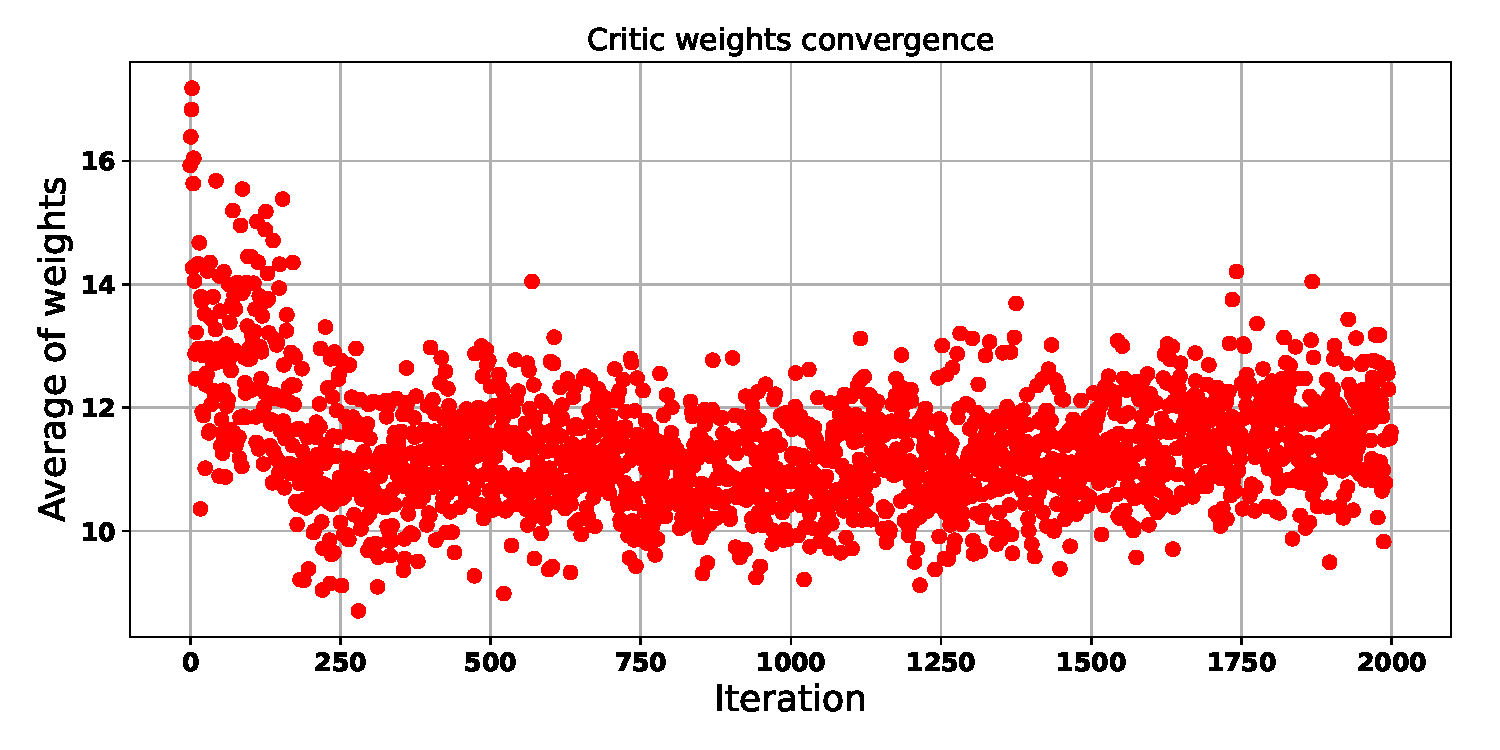
\includegraphics[width=\linewidth]{Figures/Q-value_convergence.pdf}
%     \caption{Convergence of the network weights ($\vert \vert \theta \vert \vert$) recorded at intervals of 50 iterations.}
%     \Description{Convergence of training weights over iterations.}
%     \label{fig:critic}
% \end{figure}

% Akhilesh, gave this heading to this subsection
\subsection{RL Model Evaluation}\label{sec:model_eval}
We evaluate the trained model by running it alongside test applications that the training phase has not encountered before, as well as some applications with phases (to evaluate adaptability). During evaluation, the Q-network computes the action $Q$-values corresponding to the observed state provided by the daemon process and takes the greedy action, that is, $PCAP = \arg\max_a(Q(s, a))$. This $PCAP$ is deployed by using the $RAPL$ actuators and is maintained at a steady throughput throughout the sampling interval. The sampling interval plays an important role in determining the adaptability of the controller during actuation. In our experiments we have intentionally kept the sampling interval smaller to detect minute changes in performance.
% The controller performs the informed decision making by observing the state variables thereby bringing down the overall power consumption by avoiding wastage as detailed in the section \ref{ch4:sec:Related}.

% In our case the $progress(t)$ defined in Section \ref{ch4:subsec:Performance_Measurement} depicts the state of the system at time $t$. We randomly sample action $a(t)$ from the action space $\mathcal{A}$ and observe the changes it brings to the state $progress(t)$. Following that we record the next state, $progress(t+1)$ and also calculate the reward function $r(t+1)$ at the same time.

% We use fitted Q-learning for training our agent, where data points are randomly sampled from the dataset to train the actor network. This method works best for a finite set of state action pairs. Therefore in this paper, we use a finite set of discrete actions, $\mathcal{A}$ from which the random actions are sampled to generate the dataset. The actor network is trained during each iteration of the learning phase, with a finite set of data, sampled randomly from this dataset.


% \begin{figure*}[!htb]
%     \centering
%     \newlength{\figureheight}
%     \newlength{\figurewidth}
%     \setlength{\figureheight}{5cm}
%     \setlength{\figurewidth}{9cm}
%     % First row
%     \begin{subfigure}{0.5\linewidth}
%         \centering        \includegraphics[width=\figurewidth,height=\figureheight,keepaspectratio]{Figures/repeat_fig_ones-stream-full.pdf}
%         \caption{STREAM-FULL}
%         \label{fig:stream-full-1}
%     \end{subfigure}\hfill
%     \begin{subfigure}{0.5\linewidth}
%         \centering
%         \includegraphics[width=\figurewidth,height=\figureheight,keepaspectratio]{Figures/repeat_fig_phases-stream-full.pdf}
%         \caption{PHASES-FULL}
%         \label{fig:phases-full}
%     \end{subfigure}
    
%     % Second row
%         \begin{subfigure}{0.5\linewidth}
%         \centering        \includegraphics[width=\figurewidth,height=\figureheight,keepaspectratio]{Figures/repeat_fig_ones-stream-scale.pdf}
%         \caption{STREAM-SCALE}
%         \label{fig:stream-scale}
%     \end{subfigure}\hfill
%     \begin{subfigure}{0.5\linewidth}
%         \centering        \includegraphics[width=\figurewidth,height=\figureheight,keepaspectratio]{Figures/repeat_fig_ones-stream-copy.pdf}
%         \caption{STREAM-COPY}
%         \label{fig:stream-copy}
%     \end{subfigure}
    
%     % Third row
%     \begin{subfigure}{0.5\linewidth}
%         \centering        \includegraphics[width=\figurewidth,height=\figureheight,keepaspectratio]{Figures/repeat_fig_ones-stream-add.pdf}
%         \caption{STREAM-ADD}
%         \label{fig:stream-add}
%     \end{subfigure}\hfill
%     \begin{subfigure}{0.5\linewidth}
%         \centering        \includegraphics[width=\figurewidth,height=\figureheight,keepaspectratio]{Figures/repeat_fig_ones-stream-triad.pdf}
%         \caption{STREAM-TRIAD}
%         \label{fig:stream-triad}
%     \end{subfigure}

%     % Fourth row
%     \begin{subfigure}{0.5\linewidth}
%         \centering        \includegraphics[width=8cm,height=2.8cm]{Figures/repeat_fig_ones-npb-ep.pdf}
%         \caption{NPB-EP}
%         \label{fig:npb-ep}
%     \end{subfigure}\hfill
%     \begin{subfigure}{0.5\linewidth}
%         \centering        \includegraphics[width=\figurewidth,height=\figureheight,keepaspectratio]{Figures/repeat_fig_ones-npb-is.pdf}
%         \caption{NPB-IS}
%         \label{fig:npb-is}
%     \end{subfigure}
    
%     \caption{Power vs instantaneous performance of different applications on an Intel Cascadelake processor.}
%     \label{fig:comparison}
%     \Description{Motivating example}
% \end{figure*}

% \begin{figure*}
% \begin{subfigure}{0.5\textwidth}
%         \centering
%         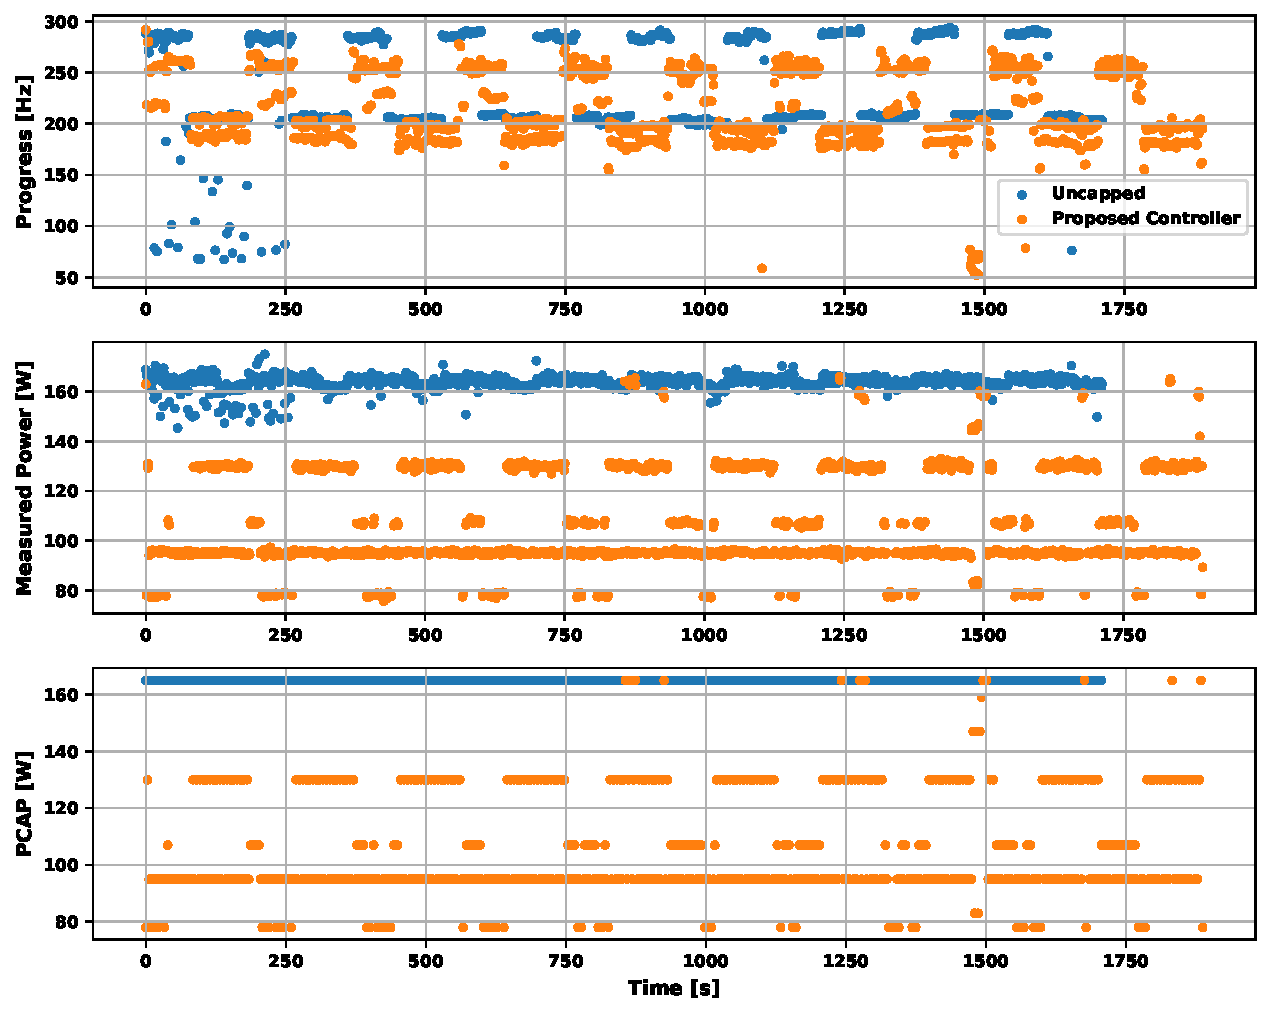
\includegraphics[width=\textwidth]{Figures/phases-stream-full.pdf} % first figure itself
%         \caption{\small{Time series plot of a single execution of STREAM application with phases showing a) progress, b) Measured Power and c) PCAP values for controlled and uncontrolled cases.}}
%         \label{fig:phases}
%     \end{subfigure}\hfill
%     \begin{subfigure}{0.5\textwidth}
%         \centering
%         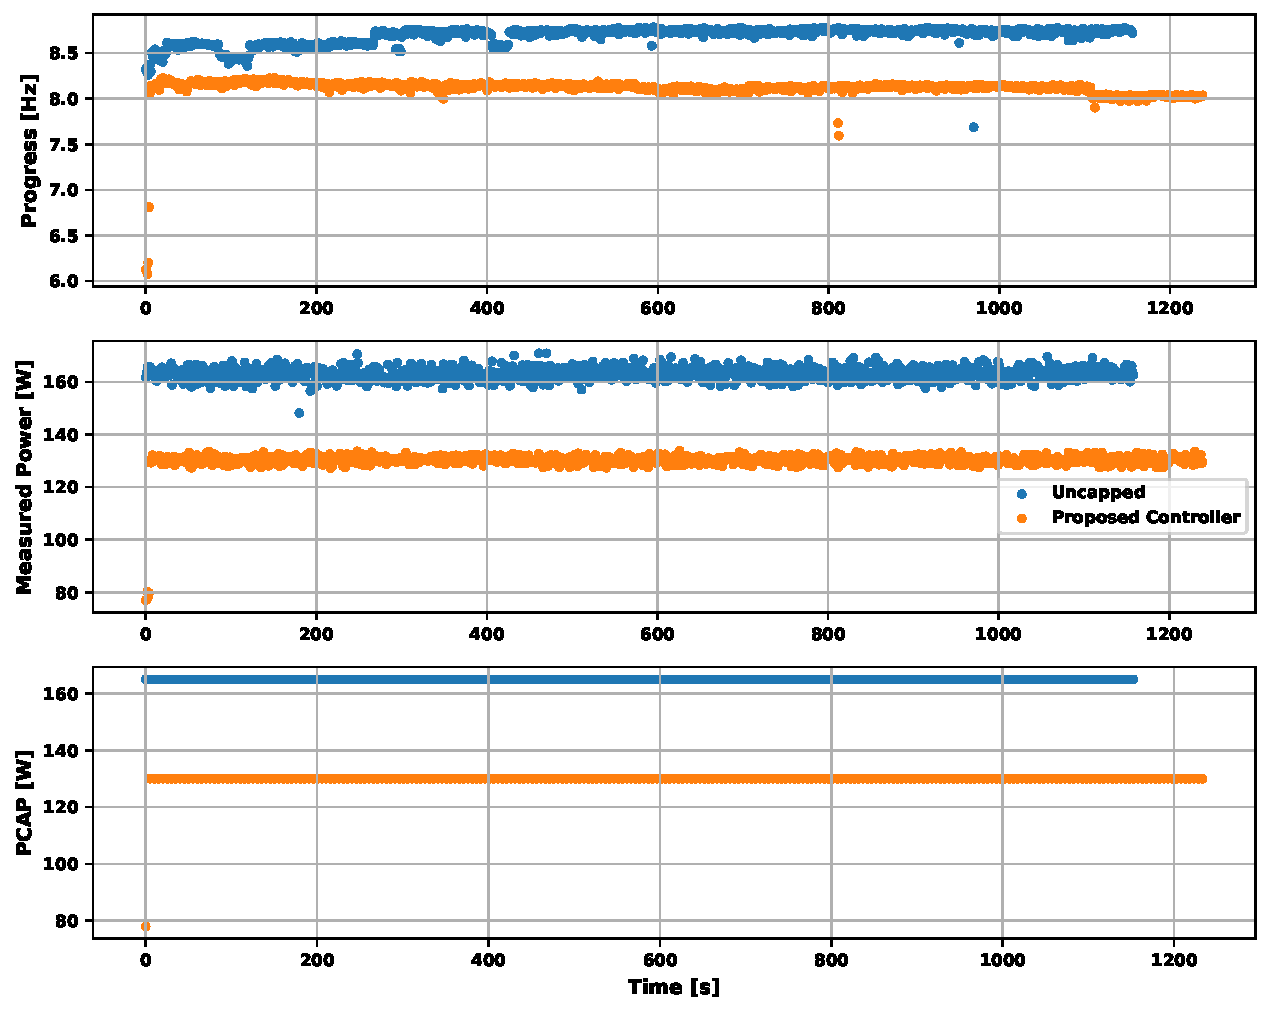
\includegraphics[width=\textwidth]{Figures/ones-npb-is.pdf} % first figure itself
%         \caption{\small{Time series plot of a single execution of $npb-is$ a compute bound application showing a) progress, b) Measured Power and c) PCAP values for controlled and uncontrolled cases.}}
%     \label{fig:npb_is}
%     \end{subfigure}
%     \Description{Application with phases}
% \end{figure*}

% \begin{figure*}[!htp]
% \centering
%     \includegraphics[width=\linewidth]{Figures/repeat_comparison.pdf}
%     \caption{Repeatability experiments performed across the same hardware node running the different benchmark applications.}
% \end{figure*}



% \begin{table*}[htbp]
% \caption{Execution time and energy consumption of all benchmark applications under three different power cap strategies (static minimum cap, static maximum cap, and our trained agent). Averages and standard deviation over 10 executions for each benchmark.}
% \begin{center}
% \resizebox{0.9\textwidth}{!}{%
% \begin{tabular}{|c|c|c|c|c|c|c|c|c|c|c|c|c|}
% \hline
% \multirow{1}{*}{benchmark applications} &
% \multicolumn{4}{c|}{Min pcap} & \multicolumn{4}{c|}{Max pcap} & \multicolumn{4}{c|}{RL} \\
% \cline{2-13}
% &\multicolumn{2}{c|}{execution time}&\multicolumn{2}{c|}{energy}&\multicolumn{2}{c|}{execution time}&\multicolumn{2}{c|}{energy}&\multicolumn{2}{c|}{execution time}&\multicolumn{2}{c|}{energy}
% \\
% \cline{2-13}
% &$\mu[\unit{\second}]$&$\sigma$&$\mu[\unit{\kilo \joule}]$&$\sigma$&$\mu[\unit{\second}]$&$\sigma$&$\mu[\unit{\kilo \joule}]$&$\sigma$&$\mu[\unit{\second}]$&$\sigma$&$\mu[\unit{\kilo \joule}]$&$\sigma$
% \\
% \hline
% {STREAM-add} & 61.56 & 0.96 & 4.81 & 0.08 & 50.40 & 2.62 & 7.84 & 0.37 & 51.17 & 0.55 & 5.66 & 0.07 \\
% \hline
% {STREAM-copy} & 43.89 & 0.57 & 3.42 & 0.04 & 35.50 & 0.81 & 5.66 & 0.12 & 38.83 & 0.69 & 3.57 & 0.08 \\
% \hline
% {STREAM-scale} & 44.45 & 0.89 & 3.46 & 0.07 & 34.40 & 1.62 & 5.59 & 0.25 & 39.08 & 1.11 & 3.58 & 0.07 \\
% \hline
% {STREAM-triad} & 64.10 & 4.04 & 4.99 & 0.31 & 50.80 & 2.82 & 7.93 & 0.40 & 51.42 & 0.86 & 5.70 & 0.11 \\
% \hline
% {STREAM-full} & 288.60 & 42.10 & 22.45 & 3.27 & 222.40 & 33.12 & 34.99 & 4.77 & 180.50 & 1.44 & 22.78 & 0.18 \\
% \hline
% {NPB-EP} & 104.30 & 4.92 & 8.12 & 0.39 & 73.80 & 4.17 & 10.33 & 0.45 & 71.10 & 1.37 & 9.08 & 0.17 \\
% \hline
% {NPB-IS} & 164.75 & 1.30 & 12.83 & 0.13 & 117.33 & 1.25 & 18.99 & 0.16 & 125.80 & 0.98 & 16.18 & 0.14 \\
% \hline
% {PHASES-STREAM-FULL} & 109.89 & 1.66 & 8.56 & 0.14 & 83.00 & 0.45 & 13.48 & 0.07 & 93.40 & 1.11 & 9.68 & 0.15 \\
% \hline
% \end{tabular}
% }
% \label{tab:repeatability}
% \end{center}
% \end{table*}
% \todo{add improvement/degradation to RL execution and energy to table}

% \begin{table*}[htbp]
% \caption{Execution time and energy consumption of all benchmark applications under three different power cap strategies (static minimum cap, static maximum cap, and our trained agent). Averages and standard deviation over 10 executions for each benchmark, including percentage degradation in execution time and percentage reduction in energy consumption under RL with respect to the Max PCAP.}
% \begin{center}
% \resizebox{\textwidth}{!}{%
% \begin{tabular}{|c|c|c|c|c|c|c|c|c|c|c|c|c|c|c|}
% \hline
% \multirow{3}{*}{benchmark applications} & \multicolumn{4}{c|}{Min $PCAP$} & \multicolumn{4}{c|}{Max $PCAP$} & \multicolumn{6}{c|}{RL} \\
% \cline{2-15}
% & \multicolumn{2}{c|}{Execution Time} & \multicolumn{2}{c|}{Energy} & \multicolumn{2}{c|}{Execution Time} & \multicolumn{2}{c|}{Energy} & \multicolumn{2}{c|}{Execution Time} & \multicolumn{2}{c|}{Energy} & \multicolumn{2}{c|}{Relative to Max pcap} \\
% \cline{2-15}
% & $\mu$[\unit{s}] & $\sigma$ & $\mu$[\unit{kJ}] & $\sigma$ & $\mu$[\unit{s}] & $\sigma$ & $\mu$[\unit{kJ}] & $\sigma$ & $\mu$[\unit{s}] & $\sigma$ & $\mu$[\unit{kJ}] & $\sigma$ & \shortstack{\scriptsize{ET Degradation}  (\%)} & \shortstack{\scriptsize{Energy Saved}  (\%)} \\
% \hline
% {ONES-STREAM-ADD} & 61.56 & 0.96 & 4.81 & 0.08 & 50.40 & 2.62 & 7.84 & 0.37 & 51.17 & 0.55 & 5.66 & 0.07 & 1.53 & 27.81 \\
% \hline
% {ONES-STREAM-COPY} & 43.89 & 0.57 & 3.42 & 0.04 & 35.50 & 0.81 & 5.66 & 0.12 & 38.83 & 0.69 & 3.57 & 0.08 & 9.38 & 36.93 \\
% \hline
% {ONES-STREAM-SCALE} & 44.45 & 0.89 & 3.46 & 0.07 & 34.40 & 1.62 & 5.59 & 0.25 & 39.08 & 1.11 & 3.58 & 0.07 & 13.60 & 36.00 \\
% \hline
% {ONES-STREAM-TRIAD} & 64.10 & 4.04 & 4.99 & 0.31 & 50.80 & 2.82 & 7.93 & 0.40 & 51.42 & 0.86 & 5.70 & 0.11 & 1.22 & 28.11 \\
% \hline
% {ONES-STREAM-FULL}& 245.99 & 53.23 & 19.13 & 4.14 & 189.5 & 24.63 & 30.35 & 3.64  & 180.50 & 1.44 & 22.78 & 0.18 & -4.75 & 24.98 \\
% \hline
% {ONES-NPB-EP} & 104.30 & 4.92 & 8.12 & 0.39 & 73.80 & 4.17 & 10.33 & 0.45 & 71.10 & 1.37 & 9.08 & 0.17 & -3.66 & 12.10 \\
% \hline
% {ONES-NPB-IS} & 164.75 & 1.30 & 12.83 & 0.13 & 117.33 & 1.25 & 18.99 & 0.16 & 125.80 & 0.98 & 16.18 & 0.14 & 7.21 & 14.80
% \\
% \hline
% {PHASES-STREAM-FULL} & 109.89 & 1.66 & 8.56 & 0.14 & 83.00 & 0.45 & 13.48 & 0.07 & 93.40 & 1.11 & 9.68 & 0.15 & 12.53 & 28.19
% \\
% \hline
% \end{tabular}
% }
% \label{tab:repeatability}
% \end{center}
% \end{table*}
% \todo{add improvement/degradation to RL execution and energy to table}

% \begin{center}
% \resizebox{\textwidth}{!}{%
% \begin{tabular}{|c|c|c|c|c|c|c|c|c|c|c|c|c|c|c|}
% \hline
% \multirow{3}{*}{benchmark applications} & \multicolumn{4}{c|}{Min $PCAP$} & \multicolumn{4}{c|}{Max $PCAP$} & \multicolumn{6}{c|}{RL} \\
% \cline{2-15}
% & \multicolumn{2}{c|}{Execution Time} & \multicolumn{2}{c|}{Energy} & \multicolumn{2}{c|}{Execution Time} & \multicolumn{2}{c|}{Energy} & \multicolumn{2}{c|}{Execution Time} & \multicolumn{2}{c|}{Energy} & \multicolumn{2}{c|}{Relative to Max pcap} \\
% \cline{2-15}
% & $\mu$[\unit{s}] & $\sigma$ & $\mu$[\unit{kJ}] & $\sigma$ & $\mu$[\unit{s}] & $\sigma$ & $\mu$[\unit{kJ}] & $\sigma$ & $\mu$[\unit{s}] & $\sigma$ & $\mu$[\unit{kJ}] & $\sigma$ & \shortstack{\scriptsize{ET Degradation}  (\%)} & \shortstack{\scriptsize{Energy Saved}  (\%)} \\
% \hline
% {Stream-Add} & 62.71 & 0.70 & 4.89 & 0.06 & 48.33 & 0.47 & 7.96 & 0.08 & 59.27 & 0.75 & 4.96 & 0.25 & 22.63 & 37.68 \\
% \hline
% {Stream-Full} & 216.57 & 3.33 & 16.88 & 0.26 & 172.33 & 0.47 & 28.27 & 0.07 & 190.09 & 1.83 & 21.98 & 0.17 & 10.30 & 22.24 \\
% \hline
% {Stream-Scale} & 43.57 & 0.49 & 3.40 & 0.05 & 34.33 & 0.47 & 5.65 & 0.08 & 39.55 & 1.30 & 3.67 & 0.27 & 15.20 & 35.0 \\
% \hline
% {Stream-Copy} & 45.00 & 0.76 & 3.50 & 0.06 & 34.67 & 0.47 & 5.72 & 0.08 & 39.55 & 1.50 & 3.72 & 0.33 & 14.0 & 34.96 \\
% \hline
% {Stream-Triad} & 59.29 & 0.45 & 4.61 & 0.03 & 47.67 & 0.47 & 7.67 & 0.07 & 58.45 & 0.50 & 4.87 & 0.07 & 22.61 & 36.50 \\
% \hline
% {NPB-EP} & 96.57 & 2.61 & 7.52 & 0.20 & 67.67 & 0.47 & 9.80 & 0.06 & 80.91 & 1.78 & 8.10 & 0.18 & 19.56 & 17.34 \\
% \hline
% \hline
% {NPB-IS} & 160.57 & 0.90 & 12.49 & 0.07 & 116.67 & 1.25 & 19.17 & 0.22 & 135.64 & 1.15 & 13.61 & 0.12 & 16.26 & 29.0 \\
% \hline
% {NPB-FT} & 160.57 & 0.90 & 12.49 & 0.07 & 116.67 & 1.25 & 19.17 & 0.22 & 135.64 & 1.15 & 13.61 & 0.12 & 16.26 & 29.0 \\
% \hline
% {NPB-MG} & 160.57 & 0.90 & 12.49 & 0.07 & 116.67 & 1.25 & 19.17 & 0.22 & 135.64 & 1.15 & 13.61 & 0.12 & 16.26 & 29.0 \\
% \hline
% {Stream-Phases} & 107.29 & 1.16 & 8.35 & 0.10 & 84.33 & 0.47 & 13.83 & 0.07 & 100.27 & 0.86 & 8.80 & 0.22 & 18.90 & 36.37 \\
% \hline
% \end{tabular}
% }
% \label{tab:repeatability}
% \end{center}
% \end{table*}


% Akhilesh, I am renaming this section
%\section{Experimental Setup}\label{sec:Setup}
\section{Applying the Methodology to a Use Case}\label{sec:setup}

We now demonstrate how we have applied our approach to a concrete use case of high performance computing applications requiring effective power-performance trade-offs. 

\subsection{Experimental Hardware and Tools Used}
All the experiments in this paper, including data collection and evaluation, were performed on a bare-metal Cascadelake node from Chameleon Cloud~\cite{keahey2019chameleon}, equipped with Intel Xeon Gold 6240R processors. The node has 2 processors, each with 24 cores and 2 hyperthreads per core, and 192 GiB of memory. The L3 cache size is 35.75 MiB per processor.

Provisioning of these nodes included a fully installed and configured Global Extensible Open Power Manager (GEOPM)~\cite{eastep2017global} service (version $3.1.0$) to enable reading and writing of power sensors, but without GEOPM being configured to provide any power control policy itself. PAPI version $6.0.0$ was used to access hardware performance counters. A custom software infrastructure handles the collection of data from GEOPM, PAPI, and application heartbeats, while also providing the basis for our control policy deployment.

\subsection{Compute-intensive Workloads used in Offline RL Model Training}

We use a collection of well-established application benchmarks to represent the behaviors of various applications and their response to power capping. Table \ref{ch4:tab:performance_metrics} presents the characteristics of various benchmarks used throughout this paper, including problem size, iterations, average $IPC$, average $CMR$, average $STL$, average progress, and average execution time ($ET$) for each kernel, calculated over 10 independent runs. The benchmarks
listed here are used both for training and for validating our control agent, with some of them being kept out of our training dataset and used  only for validation. By using these well-established benchmarks, we hope to train our model to recognize and predict optimal power management strategies that will be applicable to a wide range of application behaviors.

% moved here so it appears in the right place
\begin{table*}[htb]
    \centering
    \caption{{Detailed description of our benchmarks, including their type, parameters, and average performance metrics (uncapped).}}
    \label{ch4:tab:performance_metrics}
    \resizebox{\linewidth}{!}{%
        \begin{tabular}{|c|c|c|c|c|c|c|c|c|c|}
            \hline
            \textbf{Benchmark} & \textbf{Prob Size} & \textbf{Iter.} & \textbf{Avg. IPC} & \textbf{Avg. CMR} & \textbf{Avg. STL} & \textbf{Avg. Prog.} \textbf{[\unit{Hz}]} & \textbf{Avg. ET}\textbf{[\unit{s}]} & \textbf{Avg. Energy} \textbf{[\unit{kJ}]} & \textbf{Ari. Int. (FLOPs/Byte)} \\
            \hline
            {\textbf{STREAM SCALE}}  & 33554432 & 10000 & 0.20 & 0.89 & 0.84 & 285.20 & 34.40 & 5.59 & 1.62 \\
            \hline
            {\textbf{STREAM TRIAD}}  & 33554432 & 10000 & 0.18 & 0.94 & 0.83 & 200.03 & 50.80 & 7.93 & 1.41 \\
            \hline
            {\textbf{NPB-EP}}  & Class-W & 1000 & 0.57 & 0.13 & 0.48 & 13.61 & 73.80 & 10.33 & 53.99 \\
            \hline
            {\textbf{NPB-FT}}  & Class-B & 500 & 0.82 & 0.43 & 0.296 & 13.23 & 35.10 & 45.47 & 1.53 \\
            \hline
            {\textbf{STREAM-ADD}}  & 33554432 & 10000 & 0.15 & 0.94 & 0.85 & 201.06 & 50.40 & 7.84 & 1.36 \\
            \hline
            {\textbf{STREAM-COPY}}    & 33554432 & 10000 & 0.17 & 0.89 & 0.84 & 282.43 & 35.50 & 5.66 & 1.63 \\
            \hline
            {\textbf{STREAM-FULL}}  & 33554432 & 10000 & 0.16 & 0.93 & 0.70 & 49.31 & 222.40 & 34.99 & 1.45 \\
            \hline
            {\textbf{NPB-BT}}  & Class-C & 1000 & 0.97 & 0.87 & 0.30 & 6.22 & 166.00 & 23.168 & 0.54 \\
            \hline
            \hline
            {\textbf{STREAM-PHASE}}  & 33554432 & 10000 & 0.17 & 0.91 & 0.88 & 240.16 & 83.00 & 13.48 & 1.45 \\ 
            \hline
            {\textbf{NPB-CG}}  & Class-C & 1000 & 0.49 & 0.37 & 0.62 & 9.97 & 114.00 & 14.74 & 3.61 \\
            \hline
            {\textbf{NPB-IS}}  & Class-B & 1000 & 0.50 & 0.86 & 0.68 & 8.44 & 117.33 & 18.99 & 1.21 \\
            \hline
            {\textbf{NPB-MG}}  & Class-B & 1000 & 0.47 & 0.809 & 0.54 & 40.3 & 22.23 & 55.5 & 1.45 \\
            \hline

        \end{tabular}
    }
\end{table*}

\textbf{STREAM}~\cite{McCalpin1995} is a well-known benchmark designed to
evaluate the memory bandwidth of a system. We consider six versions of this
benchmark, corresponding to its four inner kernels (add, copy, scale, and triad)
with varying arithmetic intensity, as well as one version (\texttt{full}) that
executes all four kernels as part of its outer loop. The last version, with phases,
repeats the full benchmark a number of times, resulting in changes in progress
rate and behavior across its execution. For all these versions, the input
problem size (the size of the working arrays in memory) has a direct impact on
the performance and is chosen here so that these arrays do not fit in the last
level cache on the system under study.
    
\textbf{NAS} Parallel Benchmarks (NPB) are a collection of programs
created to benchmark the performance of parallel processors using kernels that
are representative of scientific applications. 
%While NPB has many benchmarks, 
We include six of the benchmarks here: Embarrassingly Parallel (EP) for being a
representative of a compute-bound application, Integer Sort (IS) for its focus
on random memory accesses, Fourier Transform (FT) for its straining of the cache for
memory access, Multi-Grid (MG) for its computational intensity, Conjugate
Gradient (CG) for memory-intensive and irregular communication patterns, and
Block Tridiagonal (BT) for its compute intensive and irregular communication.
Our implementation is based on the NPB-3.4-OpenMP version. 

% \begin{figure}[htb]
%     \centering
%     \begin{subfigure}[b]{0.48\textwidth}  % Adjusted width to fit side by side
%         \centering
%         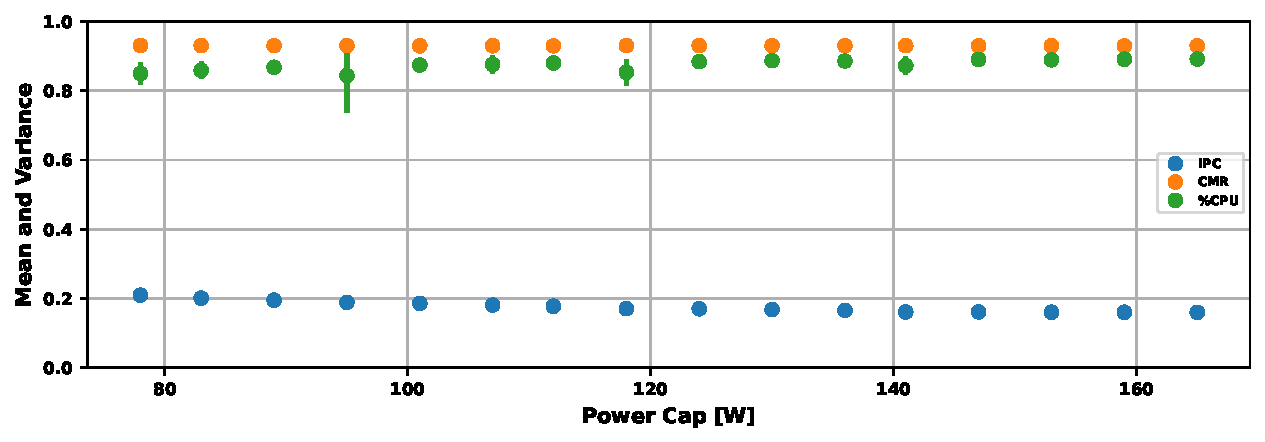
\includegraphics[width=\textwidth]{Figures/PAPI_stats_ones-stream-full.pdf}
%         \caption{$ONES-STREAM-FULL$}
%         \label{fig:stream_perf}
%     \end{subfigure}\hfill
%     \begin{subfigure}[b]{0.48\textwidth}  % Adjusted width to fit side by side
%         \centering
%         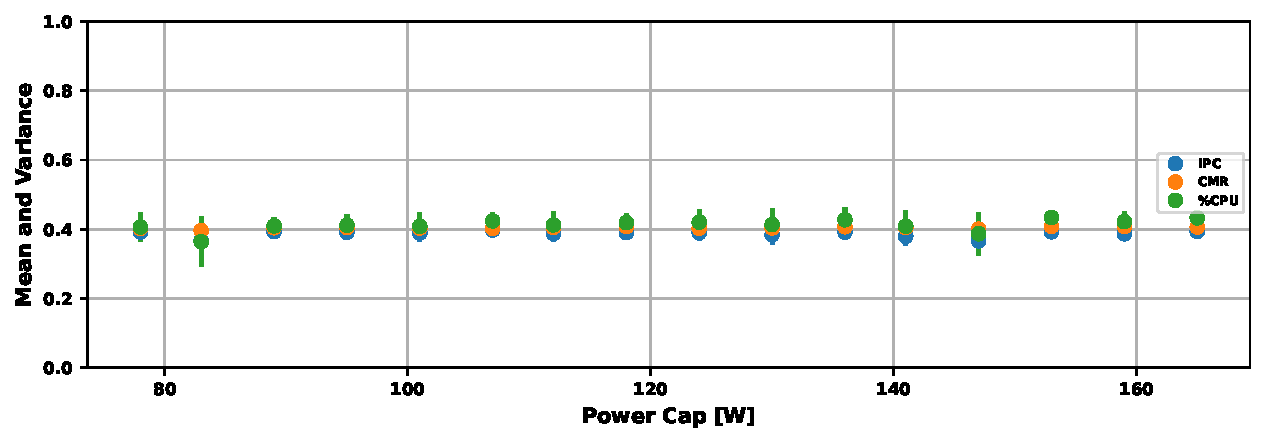
\includegraphics[width=\textwidth]{Figures/PAPI_stats_ones-npb-ep.pdf}
%         \caption{$ONES-NPB-EP$}
%         \label{fig:ep_perf}
%     \end{subfigure}
%     \caption{Average ($\mu$) and Standard deviation ($\sigma$) of IPC, CPU and CMR at various power levels for two of our benchmarks. The experiments were repeated 10 times for each of the power caps.}
%     \label{fig:mu_sigma}
%     \Description{Motivating example}
% \end{figure}


% To further motivate our use of both derived metrics and progress measurements, we generated plots for Instructions Per Cycle (IPC), CPU utilization, and Cache Miss Rate (CMR) across two distinct benchmark applications, each subjected to varying node power or Power Caps ($PCAP$s). These experiments were conducted on an Intel processor with $PCAP$s held constant during each application run. For each run, we computed the mean ($\mu$) and standard deviation ($\sigma$) of the derived metrics and charted them against their respective $PCAP$ values.
% The correlation is depicted in Figure \ref{fig:mu_sigma}. 
% To ensure consistency, we replicated the experiments 10 times for each application, keeping the problem size constant. The normalized results, illustrated in Figure \ref{fig:mu_sigma}, demonstrate unique differences in the metrics for memory-bound and compute-bound applications respectively.
% The $IPC$, $STL$, and $CMR$ values collectively constitute a distinctive vector, serving as a "fingerprint" of the application given the specific $PCAP$. Notably, the relation of performance counter metrics to $PCAP$ differs from the application's "progress" as seen in Figure \ref{fig:motivation_fig}.
% This observation underscores the insights of Ramesh et al. \cite{ramesh2019understanding}, highlighting the significance of measuring application progress towards achieving scientific objectives.
We modified these benchmarks to be iterative so that application progress is more easily identifiable: When not already a part of the benchmark, an outer loop is introduced, repeating their kernels a configurable amount of time. Each outer loop also contains our instrumentation for heartbeats, resulting in each  benchmark reporting one heartbeat per iteration. Note that the progress rate of each benchmark is different and depends on the runtime of its kernel.
% Table \ref{ch4:tab:performance_metrics} shows the names and associated characteristics of the applications we consider in this paper for a quick reference. 

Since this paper is concerned with demonstrating energy efficiency, we select each benchmark problem size to be bigger than caches, with the goal of exhibiting performance trade-offs between CPU power capping (and the resulting frequency variation) and stable memory performance.
These problem size values are provided in Table~\ref{ch4:tab:performance_metrics}. The table also provides information on the arithmetic intensity for each application, defined as the ratio between total computational operations  and total instructions, which serves as a measure of computational diversity among the applications. A double line  in the table separates applications that are part of the training dataset (top) and those used only during validation (bottom).

\subsection{Data Collection and Offline Training}


We collect our training dataset by executing each benchmark under a structured stochastic control policy and sampling all measurements that constitute the state vector during execution. Prior work in offline reinforcement learning suggests that randomly generated datasets can be sufficient to recover near-optimal policies \cite{levine2020offline}. However, uniformly random sampling over the action space can lead to sub-optimal learned policies.

To address this, we employ a weighted sampling strategy based on a Gaussian-shaped random walk over the discrete $PCAP$ action space rather than uniform sampling. At fixed control intervals, the next power cap is sampled from a Gaussian distribution centered at the constant action index, thereby inducing smooth transitions between neighboring power levels. The smoothness parameter ($\sigma$) controls the locality of exploration. For memory-bound applications such as \texttt{stream}, the operating point was selected at $89.0$ W with $\sigma = 2$, since empirical profiling shows that application progress begins to saturate near this power cap. 

To ensure that the training dataset fits the conditions under which the trained controller will operate, we set up the experiments  to sample at the same rate as the control will activate: 1 Hz (once per second). In this paper we use a random control policy during data collection: $PCAP$ values for RAPL, chosen randomly from a discretization of the action space of allowed power caps for the system. Indeed, while the system allows for a power capping range of 78 \unit{\watt} to 165 \unit{\watt}, we apply only 16 values distributed uniformly in that range. By reducing the action state to such a small and finite set of actions, we avoid the need for a much larger Q-Network (in the output dimension)
to train. This choice also significantly reduces the size of the  training dataset while preserving the controller’s performance. We ensure in our data collection that all 16 possible power caps are sampled, since CQL, like most RL algorithms, does not extrapolate on the action space observed. Nevertheless, not all transitions between two actions corresponding to all state observations are present in the dataset. 

This collection strategy is repeated for each of the benchmarks selected as part of the training set for the problem size and iterations given in  Table \ref{ch4:tab:performance_metrics}. To ensure an independent and identically distributed (i.i.d.) dataset across applications, we execute applications with lower average execution times more frequently than others. Rewards are computed from these state vectors and appended to the dataset and normalized as explained in Section~\ref{ch4:sec:Methodology}.

% The action space consists of a set of finite actions allowed by the Global Extensible Open Power Manager (GEOPM) \cite{eastep2017global}, which is a software framework to explore power and energy optimizations on platforms with heterogeneous mixes of computing hardware. Our motive, as defined in Section \ref{ch4:sec:Introduction}, being identifying the maximum efficiency point of operation for the application on an HPC node, will be represented by the reward function as a function of the application progress and power consumption.
In our case the state variable at time  $t$, $s(t)$ consists of the progress of the system, the measured power (the measure of how much of the supplied power is being utilized) and the characteristics of the application. 

\begin{equation*}
s(t) = [progress(t), P_{avg}(t), IPC(t), STL(t), CMR(t)].
\end{equation*}
The action is the CPU power supplied using the RAPL actuators, that is, $a(t) = PCAP(t)$. Upon observing $s(t)$ the system transitions to $s(t+1)$ under the action $a(t)$ following the transition dynamics under the policy.

The resulting dataset consists of filtered data points ($s(t), a(t), r(t+1), s(t+1)$),  on which offline training is performed. Since the action space is finite, we use a Q-network consisting of output dimensions equivalent to the cardinality of the action space (i.e., 16). The input dimension is the dimension of the state space or observation space, which is 5. The 2 intermediate layers consist of 20 neurons each. A total of 10,000 iterations, with a discount factor $\gamma = 0.9$ and the CQL constant $\alpha = 0.1$, was used for training, with a buffer size of 128. It is recommended to keep the $\alpha$ at larger values ( 0.3) for larger datasets to compensate for out-of-distribution observations. The number of iterations is chosen based on the time it takes for the Q-network to converge.

